\documentclass[11pt]{article}
\usepackage[margin=2.5cm]{geometry}
\usepackage{booktabs}
\usepackage{tabularx}
\usepackage{graphicx}
\usepackage{enumitem}
\usepackage{float}
\usepackage[bidi=basic, layout=tabular.lists.captions]{babel}
\babelprovide[main, import]{hebrew}
\babelprovide[import]{english}
\babelfont{rm}{Times New Roman}
\babelfont{tt}{Courier New}
\usepackage[hidelinks]{hyperref}
\setlist[description]{leftmargin=2.4cm, labelwidth=2.2cm, itemsep=2pt, font=\normalfont\itshape}
\newcommand{\en}[1]{\foreignlanguage{english}{#1}}

\title{מאגרי נתונים לסיווג תתי-גרפים:\\ שבעת המאגרים שנבחרו}
\author{}
\date{11 באוקטובר 2026}

\begin{document}
\maketitle

\section*{מה אנחנו מחפשים}

אנחנו מסווגים ישות, שאנחנו קוראים לה \emph{צבע}, לפי תת-הגרף שלה בתוך גרף גדול אחד. בנתוני
ההריון שלנו צומת הוא ביקור אחד, תת-גרף הוא כל הביקורים של מטופלת אחת, והתווית אומרת אם
למטופלת היה התוצא. יש $61{,}046$ ביקורים, $6{,}590$ מטופלות, ו-$11\%$ מהן חיוביות. הקשתות
מחברות ביקורים עם טקסט דומה ($20$ שכנים לכל ביקור).

מאגר מתאים אם יש בו ארבעה דברים. כל צומת שייך לתת-גרף אחד בדיוק, ובכל תת-גרף יש צמתים רבים.
יש תווית אחת לכל תת-גרף, רצוי בינארית. הקשתות נבנות מטקסט או מווקטורים של הצמתים, או ניתנות
על ידי המקור. ואי אפשר לנחש את התווית מגודל תת-הגרף בלבד.

מתוך $14$ המועמדים בגרסה הראשונה של הדוח נבחרו שבעה: \en{JODIE Reddit}, \en{Synthea 1k},
\en{Synthea 5k}, \en{Deezer Europe}, \en{CaLiGraph}, \en{Amazon}, ו-\en{Gene Ontology} עם
\en{STRING}. הגרסה הזו מתארת כל אחד מהם בפירוט. שלושה כבר בנויים; ארבעת האחרים לא.

\section*{במבט אחד}

\begin{table}[H]
\centering
\small
\begin{tabularx}{\textwidth}{lXXXl}
\toprule
מאגר & צומת & תת-גרף (צבע אחד) & התווית של תת-הגרף & מצב \\
\midrule
הריון (שלנו) & ביקור & הביקורים של מטופלת & היה התוצא & קיים \\
\addlinespace
\en{JODIE Reddit} & פוסט & הפוסטים של משתמש & המשתמש נחסם & נבנה \\
\en{Synthea 1k / 5k} & ביקור & הביקורים של מטופל & למטופל יש סוכרת & נבנה \\
\en{Deezer Europe} & משתמש & קבוצת משתמשים (לבחירה) & רוב ממגדר אחד או לא & הורד \\
\en{CaLiGraph} & ישות & הישויות של מחלקה אחת & תחת מחלקת-אב או לא & עוד לא \\
\en{Amazon} & מוצר & המוצרים של קטגוריה אחת & ספרים או לא & עוד לא \\
\en{GO + STRING} & חלבון & החלבונים של מונח \en{GO} אחד & תחת מונח-אב או לא & עוד לא \\
\bottomrule
\end{tabularx}
\caption{איך כל מאגר מתחלק לתתי-גרפים ומה התווית של כל תת-גרף. בארבעת האחרונים הקיבוץ והתווית
הם ההצעה שלנו.}
\end{table}

\section*{מקום בדיסק}

\begin{table}[H]
\centering
\small
\begin{tabular}{lrrl}
\toprule
מאגר & הורדה & בדיסק, פרוס & מקור המספר \\
\midrule
\en{JODIE Reddit} & \en{2.3 GB} & \en{2.3 GB} & נמדד, כבר במחשב הזה \\
\en{Synthea 1k} & תוכנה של \en{188 MB} & \en{226 MB} & נמדד, כבר במחשב הזה \\
\en{Synthea 5k} & (אותה תוכנה) & \en{1.1 GB} & נמדד, כבר במחשב הזה \\
\en{Deezer Europe} & \en{2.6 MB} & \en{7.5 MB} & נמדד \\
\en{CaLiGraph} & \en{1.4 GB} (\en{3.8 GB} לכל הקבצים) & בערך \en{10--15 GB} & ההורדה נמדדה, השאר הערכה \\
\en{Amazon} & \en{221 MB} & בערך \en{1 GB} & ההורדה נמדדה, השאר הערכה \\
\en{GO + STRING} & בערך \en{200 MB} & בערך \en{1 GB} & ההורדה נמדדה, השאר הערכה \\
\midrule
סך הכול & \en{4.3 GB} & בערך \en{16--21 GB} & \\
\bottomrule
\end{tabular}
\caption{המקום שדרוש לקבצים הגולמיים. גודלי ההורדה נלקחו מהשרתים ב-11 באוקטובר 2026. הגודל
הפרוס של הקבצים שעוד לא הורדו הוא הערכה. ההורדה החדשה היא בערך \en{1.8 GB} אם לא סופרים שוב את
\en{JODIE} ו-\en{Synthea}, שכבר נמצאים כאן.}
\end{table}

\paragraph{רק \en{CaLiGraph} גדול.} הקבצים שלו הם טקסט דחוס שגדל בערך פי עשרה כשפורסים אותו. אפשר
גם לקרוא אותם בלי לפרוס, וכך הוא נשאר \en{1.4 GB}.

\paragraph{גרפים בנויים דורשים מקום נוסף.} הגרף המעובד של \en{JODIE Reddit} תופס \en{649 MB},
ושל \en{Synthea} \en{130 MB} (\en{1k}) ו-\en{632 MB} (\en{5k}). גרף מעובד גדל עם מספר הצמתים, ולכן
\en{CaLiGraph}, עם מיליוני ישויות, ידרוש הרבה \en{GB} אם לא נשאיר רק חלק ממנו.

\section*{שלושת המאגרים הבנויים}

המספרים לקוחים מהבנייה שלנו.

\begin{table}[H]
\centering
\small
\begin{tabular}{lrrrrrr}
\toprule
 & תתי-גרפים & חיוביים & גודל ממוצע & חציון & הקטן--הגדול & גודל, חיובי / שלילי \\
\midrule
הריון (שלנו) & $6{,}590$ & $11.4\%$ & $9.3$ & $5$ & \en{2--221} & \en{8.3 / 9.4} \\
\en{JODIE Reddit} & $10{,}000$ & $3.7\%$ & $67.2$ & $44$ & \en{29--4,690} & \en{61.1 / 67.5} \\
\en{Synthea 1k} & $1{,}160$ & $14.5\%$ & $58.0$ & $36$ & \en{1--810} & \en{\textbf{166.1} / 39.8} \\
\en{Synthea 5k} & $5{,}678$ & $14.6\%$ & $57.4$ & $36$ & \en{1--866} & \en{\textbf{164.8} / 39.0} \\
\bottomrule
\end{tabular}
\caption{גודל ואיזון התוויות של תתי-הגרפים. גודל הוא מספר הצמתים בתת-גרף. העמודה האחרונה היא
הגודל הממוצע של תתי-גרפים חיוביים ושל שליליים.}
\end{table}

\begin{table}[H]
\centering
\small
\begin{tabular}{lrrrr}
\toprule
 & חלקים לתת-גרף & קשתות בתוך תת-גרף & \multicolumn{2}{c}{שכנים עם אותה תווית} \\
 & (ממוצע) & (חלק מכל הקשתות) & נצפה & באקראי \\
\midrule
הריון (שלנו) & $8.8$ מתוך $9.3$ & $0.4\%$ & $83.0\%$ & $81.7\%$ \\
\en{JODIE Reddit} & $45.9$ מתוך $67.2$ & $10.5\%$ & $93.7\%$ & $93.6\%$ \\
\en{Synthea 1k} & $47.7$ מתוך $58.0$ & $5.8\%$ & $79.4\%$ & $51.5\%$ \\
\en{Synthea 5k} & $52.5$ מתוך $57.4$ & $2.1\%$ & $79.9\%$ & $51.3\%$ \\
\bottomrule
\end{tabular}
\caption{איך תתי-הגרפים יושבים בגרף. \emph{חלקים} הוא מספר החלקים הקשירים של תת-גרף כשמשאירים
רק את הקשתות שלו (מתוך מספר הצמתים בו). \emph{שכנים עם אותה תווית} מסתכל על קשתות בין שני
תתי-גרפים שונים ושואל כמה פעמים לשניהם אותה תווית; \emph{באקראי} הוא מה שהיינו רואים אם הקשתות
האלה היו מונחות באקראי.}
\end{table}

\paragraph{תתי-הגרפים שלנו קטנים בהרבה.} למטופלת בהריון יש בממוצע $9$ ביקורים. למשתמשים
ולמטופלים ב-\en{JODIE} וב-\en{Synthea} יש בערך $60$.

\paragraph{ב-\en{Synthea} הגודל מסגיר את התווית.} למטופלים חיוביים יש בערך פי ארבעה ביקורים
($165$ לעומת $39$). ב-\en{JODIE Reddit} ובנתונים שלנו לשתי התוויות יש בערך אותו גודל.

\paragraph{תתי-הגרפים לא קשירים מבפנים.} מטופלת עם $9.3$ ביקורים מתפרקת ל-$8.8$ חלקים נפרדים.
\en{JODIE} ו-\en{Synthea} קשירים קצת יותר, אבל עדיין רובם בחלקים.

\paragraph{רק ב-\en{Synthea} יש אות תווית בקשתות.} ב-\en{JODIE Reddit} ובנתונים שלנו, תתי-גרפים
שכנים חולקים תווית לא יותר מאשר במקרה. ב-\en{Synthea} הם חולקים אותה ב-$80\%$ מהפעמים לעומת
$51\%$ במקרה, ושוב ייתכן שזה בא מהגודל.

\begin{figure}[H]
\centering
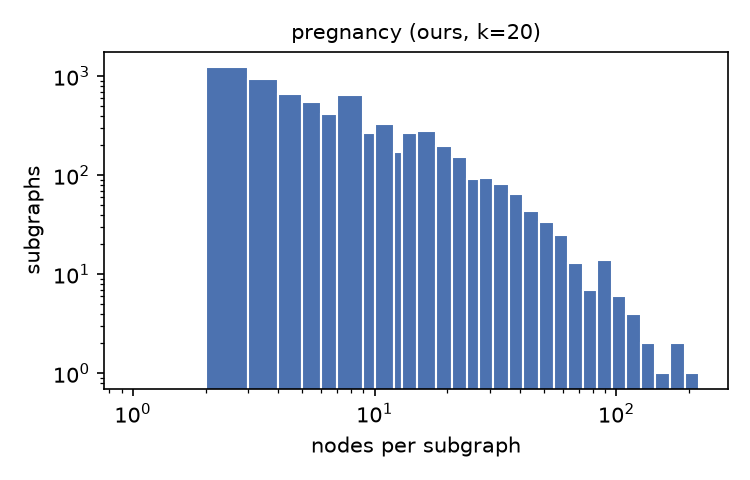
\includegraphics[width=.48\textwidth]{figures/sizes_pregnancy_ours_k_20.png}
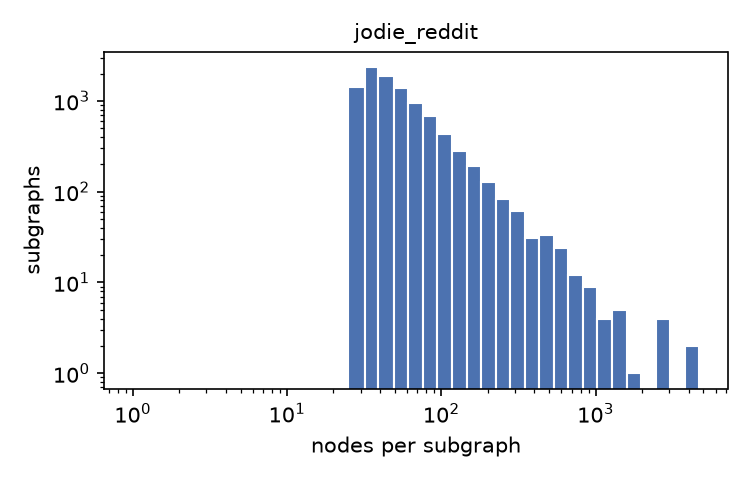
\includegraphics[width=.48\textwidth]{figures/sizes_jodie_reddit.png}\\[4pt]
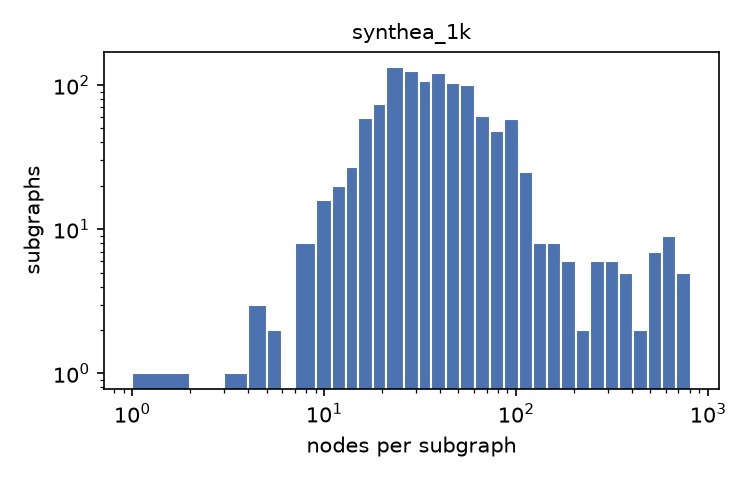
\includegraphics[width=.48\textwidth]{figures/sizes_synthea_1k.png}
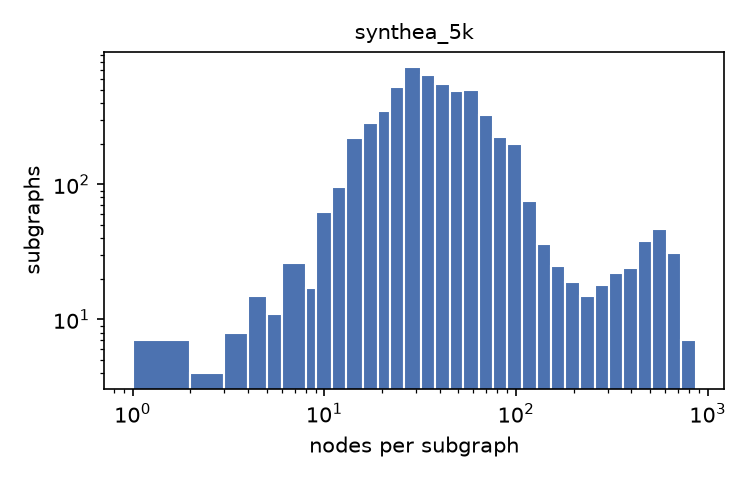
\includegraphics[width=.48\textwidth]{figures/sizes_synthea_5k.png}
\caption{מספר תתי-הגרפים בכל גודל, בצירים לוגריתמיים. ל-\en{Synthea} יש גבעה שנייה של מטופלים
גדולים מאוד, בין $200$ ל-$900$ ביקורים.}
\end{figure}

\clearpage
\section*{כל מאגר בפירוט}

\subsection*{\en{JODIE Reddit}}

מהמאמר של \en{JODIE} (\en{Kumar, Zhang and Leskovec, KDD 2019}). הוא מתעד חודש אחד של פוסטים של
$10{,}000$ המשתמשים הפעילים ביותר ב-\en{Reddit}, ב-$984$ ה-\en{subreddits} (פורומים לפי נושא)
הפעילים ביותר.

\begin{description}
\item[מקור] \href{http://snap.stanford.edu/jodie/reddit.csv}{\en{snap.stanford.edu/jodie}}, קובץ
אחד, \texttt{\en{reddit.csv}}, \en{2.3 GB}. כבר נמצא ב-\texttt{\en{data/raw/jodie\_reddit}}.
\item[צומת] פוסט אחד. יש $672{,}447$ פוסטים. כל שורה נותנת את המשתמש, ה-\en{subreddit}, הזמן
ודגל חסימה.
\item[וקטור צומת] $172$ מספרים שנוצרו מטקסט הפוסט בעזרת \en{LIWC}, כלי שסופר מילים לפי קטגוריה
(למשל מילים עצובות או מילים על משפחה). הטקסט עצמו לא כלול, ולכן אי אפשר להטמיע אותו בדרך שלנו.
\item[קשתות] לא ניתנות. אנחנו מחברים כל פוסט ל-$20$ הפוסטים הדומים לו ביותר לפי הווקטורים האלה,
ומקבלים $10.5$ מיליון קשתות.
\item[תת-גרף] כל הפוסטים של משתמש אחד. לכל משתמש יש לפחות $29$ פוסטים.
\item[תווית] $1$ אם המשתמש נחסם ב-\en{subreddit} בשלב כלשהו, אחרת $0$. רק $366$ משתמשים
($3.7\%$) חיוביים.
\item[לא בשימוש] ה-\en{subreddit} והזמן של כל פוסט נמצאים בקובץ אבל לא בגרף שלנו.
\item[בעיות] התווית נדירה, ובווקטורי \en{LIWC} יש מעט אות תווית: שכנים חולקים תווית לא יותר
מאשר במקרה.
\end{description}

\subsection*{\en{Synthea 1k} ו-\en{5k}}

\en{Synthea} היא תוכנה שממציאה רשומות רפואיות מציאותיות (קוד פתוח, של \en{MITRE}). לא מורידים
דבר מלבד התוכנה; הרשומות נוצרות אצלנו.

\begin{description}
\item[מקור] \href{https://github.com/synthetichealth/synthea}{\en{github.com/synthetichealth/synthea}},
קובץ \en{Java} אחד של \en{188 MB}. הרשומות נוצרות עם \en{seed} $42$ עבור $1{,}000$ ו-$5{,}000$
אנשים חיים. אנשים שמתים בדרך נשמרים גם הם, ולכן מתקבלים $1{,}160$ ו-$5{,}678$ מטופלים.
\item[קבצים] שבע טבלאות בכל הרצה: מטופלים, ביקורים, מצבים רפואיים, תרופות, פרוצדורות, בדיקות
מעבדה וחיסונים. טבלת הבדיקות היא הגדולה ביותר (\en{145 MB} מתוך \en{226 MB} ב-\en{1k}).
\item[צומת] ביקור אחד: $67{,}331$ ב-\en{1k} ו-$325{,}760$ ב-\en{5k}.
\item[טקסט צומת] נבנה מהביקור: הסוג והסיבה שלו, ואחריהם האבחנות, הפרוצדורות, התרופות, החיסונים
והבדיקות. כל אזכור של סוכרת ושל התרופות שלה מוסר. הטקסט מוטמע באותו מודל משפטים קטן כמו קודם
(\en{MiniLM}).
\item[קשתות] כל ביקור מחובר ל-$20$ הביקורים הדומים לו ביותר לפי הטקסט.
\item[תת-גרף] כל הביקורים של מטופל אחד.
\item[תווית] $1$ אם למטופל יש מצב כלשהו של סוכרת (לא כולל טרום-סוכרת), אחרת $0$. בערך $15\%$
חיוביים.
\item[בעיות] למטופלים חיוביים יש פי ארבעה ביקורים, ולכן הגודל לבדו מנבא את התווית. רשומות
סינתטיות גם סדירות יותר מרשומות אמיתיות. קיימת גם הרצה של \en{20k} (\en{4.5 GB}), אבל היא לא
נבחרה.
\end{description}

\subsection*{\en{Deezer Europe}}

רשת חברתית של משתמשי שירות המוזיקה \en{Deezer}, שנאספה במרץ 2020 עבור המאמר \en{FEATHER}
(\en{Rozemberczki and Sarkar, 2020}). הורדנו אותה כדי לבדוק את הקבצים.

\begin{description}
\item[מקור] \href{https://snap.stanford.edu/data/feather-deezer-social.html}{\en{SNAP}}, קובץ
\en{zip} אחד של \en{2.6 MB} עם שלושה קבצים: קשתות (\en{1.0 MB}), מאפיינים (\en{6.2 MB}) ותוויות
(\en{0.2 MB}).
\item[צומת] משתמש אחד. יש $28{,}281$ משתמשים ממדינות באירופה.
\item[וקטור צומת] רשימת האמנים שהמשתמש אהב, $34$ בממוצע מתוך $31{,}241$ אמנים. האמנים נתונים
רק כמספרים, בלי שמות, ולכן אין טקסט.
\item[קשתות] ניתנות: $92{,}752$ מעקבים הדדיים. זה בערך $6.6$ שכנים למשתמש, לעומת $32$ בגרף שלנו.
אפשר גם לחבר משתמשים שאוהבים אותם אמנים.
\item[תווית צומת] המגדר של המשתמש, שהכותבים ניחשו לפי שם המשתמש. ל-$44\%$ מהמשתמשים יש תווית
$1$; הקבצים לא אומרים איזה מגדר זה.
\item[תת-גרף] \textbf{לא נקבע.} הגרסה הראשונה הציעה את המשתמשים של מדינה אחת, אבל בקבצים אין
מדינה. קבוצה צריכה לבוא מהגרף עצמו, למשל אשכולות של משתמשים שעוקבים זה אחרי זה או שאוהבים
אותם אמנים.
\item[תווית] $1$ אם לרוב המשתמשים בקבוצה יש תווית $1$, אחרת $0$.
\item[בעיות] התווית של תת-הגרף נוצרת ממיצוע של תוויות צמתים, ולכן היא טובה רק כמו ניחוש המגדר
לפי השם. כמה קבוצות נקבל, ובאיזה גודל, תלוי באשכול.
\end{description}

\subsection*{\en{CaLiGraph}}

גרף ידע שנבנה מקטגוריות ומדפי רשימה של ויקיפדיה על גבי האונטולוגיה של \en{DBpedia}, באוניברסיטת
מנהיים (\en{Heist and Paulheim}). יש בו יותר ממיליון מחלקות ומיליוני ישויות רבים (אנשים, מקומות,
יצירות וכן הלאה).

\begin{description}
\item[מקור] \href{https://doi.org/10.5281/zenodo.8068322}{\en{Zenodo}}, גרסה \en{3.1.1} מיוני 2023,
רישיון \en{CC BY 4.0}. אתר הפרויקט, שלא ענה ב-10 באוקטובר, ענה שוב ב-11 באוקטובר.
\item[קבצים] $13$ קבצים דחוסים בפורמט \en{N-Triples}, פורמט טקסט עם עובדה אחת בכל שורה,
\en{3.8 GB} בסך הכול. אנחנו צריכים ארבעה מהם, \en{1.4 GB}: האונטולוגיה, שמחזיקה את עץ המחלקות
(\en{32 MB}); המחלקה של כל ישות (\en{525 MB}); השם של כל ישות (\en{485 MB}); והקשרים בין ישויות
(\en{345 MB}).
\item[צומת] ישות אחת.
\item[טקסט צומת] רק שם הישות. טקסט ארוך יותר, כמו התקציר מוויקיפדיה, לא נמצא בקבצים האלה ויגיע
מ-\en{DBpedia}.
\item[קשתות] ניתנות: קשרים בין ישויות, למשל אדם והעיר שבה נולד. אפשר גם לחבר ישויות עם שמות או
טקסט דומים.
\item[תת-גרף] הישויות של מחלקה אחת. לישות יש מחלקות רבות, ולכן נשאיר את הספציפית ביותר.
\item[תווית] $1$ אם המחלקה נמצאת תחת מחלקת-אב שנבחרה (למשל \en{Person}), אחרת $0$.
\item[צפוי] בערך $10$ ישויות למחלקה בממוצע, קרוב ל-$9$ הביקורים שלנו למטופלת.
\item[בעיות] גדול מדי לשימוש כולו, ולכן צריך לחתוך חלק. שמות של מחלקות וישויות אומרים לא פעם
את המחלקה במפורש (\en{``American novelists''}), מה שעלול להפוך את התווית לקלה.
\end{description}

\subsection*{\en{Amazon}}

מוצרים שנמכרו באמזון בקיץ 2006. שני מאגרים של \en{SNAP} מכסים אותם: גרף רכישה-משותפת עם קבוצות
מוצרים (\en{Yang and Leskovec, 2012}) ופרטי המוצרים שמאחוריו.

\begin{description}
\item[מקור] \href{https://snap.stanford.edu/data/com-Amazon.html}{\en{com-Amazon}}: הגרף
(\en{4.5 MB}) והקבוצות שלו (\en{5.5 MB}).
\href{https://snap.stanford.edu/data/amazon-meta.html}{\en{amazon-meta}}: פרטי מוצרים,
\en{211 MB} דחוס.
\item[צומת] מוצר אחד. בגרף יש $334{,}863$ מוצרים; הפרטים מכסים $548{,}552$. סביר ששניהם משתמשים
באותם מספרי מוצר, אבל זה עוד לא נבדק.
\item[טקסט צומת] הכותרת של כל מוצר ומקומו בעץ הקטגוריות (למשל
\en{Books > Subjects > History}). הביקורות נותנות תאריך, דירוג כוכבים והצבעות, אבל \textbf{אין
בהן טקסט}; הגרסה הראשונה של הדוח טעתה בנקודה הזו.
\item[קשתות] ניתנות: $925{,}872$ זוגות מוצרים שנקנים לעיתים קרובות יחד. אפשר גם לחבר מוצרים עם
כותרות דומות.
\item[תת-גרף] המוצרים של קטגוריה אחת. \en{SNAP} כבר מפצל כל קטגוריה לחלקים הקשירים שלה ומשמיט
חלקים של פחות מ-$3$ מוצרים. מוצר יכול להיות בכמה קטגוריות, ולכן נשאיר אחת.
\item[תווית] $1$ אם בקטגוריה יש ספרים, אחרת $0$. ספרים הם $72\%$ מהמוצרים ($393{,}561$), אחריהם
מוזיקה ($103{,}144$), סרטי וידאו ($26{,}132$) ו-\en{DVD} ($19{,}828$). דירוג ממוצע גבוה לעומת
נמוך הוא תווית חלופית.
\item[בעיות] תווית הספרים לא מאוזנת לכיוון השני (רובם חיוביים), והכותרת ונתיב הקטגוריה עלולים
להסגיר אותה.
\end{description}

\subsection*{\en{Gene Ontology} ו-\en{STRING}}

חלבונים אנושיים. \en{STRING} נותן אילו חלבונים עובדים יחד; \en{Gene Ontology} (\en{GO}) נותן מה
כל חלבון עושה, כמונחים שמסודרים בעץ. המאגר \en{PPI-BP} של \en{SubGNN} בנוי באותה דרך:
$21{,}521$ חלבונים, $1{,}591$ תתי-גרפים של כ-$10$ חלבונים כל אחד, ו-$6$ מחלקות.

\begin{description}
\item[מקור] \href{https://version-12-0.string-db.org/cgi/download?species_text=Homo+sapiens}{\en{STRING v12}}
לאדם: קשרים (\en{79 MB}), מידע על החלבונים (\en{2 MB}), שמות במאגרים אחרים (\en{19 MB}), ושתי
קבוצות מוכנות של וקטורי חלבונים (\en{19 MB} ו-\en{36 MB}).
\href{https://geneontology.org/docs/download-go-annotations/downloads/}{\en{GO}}: קובץ האנוטציות
האנושי (\en{12 MB}) ועץ המונחים (\en{32 MB}). בערך \en{200 MB} בסך הכול.
\item[צומת] חלבון אחד, בערך $19{,}000$ ב-\en{STRING} (מהזיכרון).
\item[טקסט צומת] תיאור קצר של כל חלבון בקובץ המידע של \en{STRING}. \en{STRING} נותן גם וקטורים
שנוצרו מרצף החלבון ומהרשת.
\item[קשתות] ניתנות: זוגות חלבונים עם ציון ביטחון מ-$0$ עד $1000$. נשאיר זוגות מעל סף, למשל
$700$ (ביטחון גבוה).
\item[התאמה] \en{STRING} משתמש במזהים משלו ו-\en{GO} משתמש במזהי \en{UniProt}. קובץ השמות של
\en{STRING} ממפה בין השניים.
\item[תת-גרף] החלבונים של מונח \en{GO} אחד. לחלבון יש מונחים רבים, ולכן נשאיר אחד, או נאפשר חפיפה.
\item[תווית] $1$ אם המונח נמצא תחת ענף שנבחר בעץ של \en{GO}, אחרת $0$.
\item[בעיות] תיאורי החלבונים אומרים לא פעם את התפקיד, שקרוב לתווית. חלק ממונחי \en{GO} עצמם
הוסקו מאותו סוג של ראיות כמו קשתות \en{STRING}.
\end{description}

\end{document}
